%% ============================================================
%%  poster.tex  –  A0 portrait research poster
%%  Gas Usage Forecasting and Delivery Optimization for Scot Forge
%%  Kumar Mantha · Vandit Goel · Pratyaksh Mathur  |  April 2026
%%
%%  Requires: beamerposter, tcolorbox, tikz, booktabs, tabularx
%%  Compile with:  pdflatex poster.tex
%% ============================================================
\documentclass[final]{beamer}

\mode<presentation>{\usetheme{default}}

\usepackage[orientation=portrait,size=a0,scale=1.35]{beamerposter}

\usepackage[T1]{fontenc}
\usepackage[utf8]{inputenc}
\usepackage{lmodern}
\usepackage{graphicx}
\usepackage{booktabs}
\usepackage{tabularx}
\usepackage{amsmath}
\usepackage{xcolor}
\usepackage{enumitem}
\usepackage{microtype}
\usepackage{tcolorbox}
\usepackage{tikz}
\usepackage{array}

\usetikzlibrary{arrows.meta, positioning, shapes.geometric}
\tcbuselibrary{skins, breakable}

%% ---- Colour palette -----------------------------------------
\definecolor{navyblue}{RGB}{26,58,90}        % primary dark navy
\definecolor{steelblue}{RGB}{68,114,196}     % accent steel blue
\definecolor{lightblue}{RGB}{219,229,241}    % pale blue fills
\definecolor{offwhite}{RGB}{248,248,248}     % box backgrounds
\definecolor{darkgray}{RGB}{50,50,50}        % body text
\definecolor{resultgreen}{RGB}{45,105,45}    % improvement numbers
\definecolor{resultred}{RGB}{175,40,40}      % negative values

%% ---- Beamer overrides ---------------------------------------
\setbeamertemplate{navigation symbols}{}
\setbeamercolor{background canvas}{bg=white}
\setbeamercolor{normal text}{fg=darkgray,bg=white}
\setbeamercolor{posterheadline}{fg=white,bg=navyblue}
\setbeamercolor{posteraccent}{fg=white,bg=steelblue}
\setbeamercolor{posterfooter}{fg=lightblue,bg=navyblue}

%% ---- tcolorbox styles ---------------------------------------
%  Standard content box
\newtcolorbox{pbox}[2][]{%
  enhanced, arc=6pt, boxrule=0pt,
  top=9pt, bottom=9pt, left=12pt, right=12pt,
  colback=offwhite,
  colframe=navyblue,
  colbacktitle=navyblue,
  coltitle=white,
  fonttitle=\bfseries\large,
  title={#2},
  attach boxed title to top left={yshift=-3mm, xshift=8mm},
  boxed title style={arc=4pt, boxrule=0pt},
  #1%
}

%  Highlighted callout box
\newtcolorbox{callout}[1][]{%
  enhanced, arc=8pt, boxrule=2pt,
  top=10pt, bottom=10pt, left=14pt, right=14pt,
  colframe=steelblue, colback=lightblue,
  #1%
}

%  Dark accent box (for big KPI number)
\newtcolorbox{bigkpi}[1][]{%
  enhanced, arc=8pt, boxrule=0pt,
  top=12pt, bottom=12pt, left=12pt, right=12pt,
  colback=navyblue, colframe=navyblue,
  #1%
}

%% ---- List spacing -------------------------------------------
\setlist[itemize]{leftmargin=1.4em, itemsep=2pt, topsep=3pt, parsep=0pt}

%% ==============================================================
\begin{document}
\begin{frame}[t]{}

%% ============================================================
%% HEADER
%% ============================================================
\begin{beamercolorbox}[wd=\paperwidth, ht=13.5cm, sep=0cm]{posterheadline}
  \vspace{1.0cm}
  \centering
  {\fontsize{56}{62}\selectfont\bfseries
    Gas Usage Forecasting and Delivery Optimization for Scot Forge}\\[0.7cm]
  {\fontsize{30}{34}\selectfont
    Kumar Mantha \quad\textbullet\quad Vandit Goel \quad\textbullet\quad Pratyaksh Mathur}\\[0.5cm]
  {\fontsize{22}{26}\selectfont\color{lightblue}
    Data Analytics Capstone Project
    \quad$|$\quad Illinois Institute of Technology
    \quad$|$\quad April 2026}
\end{beamercolorbox}

%% Accent rule
\begin{beamercolorbox}[wd=\paperwidth, ht=0.55cm]{posteraccent}
\end{beamercolorbox}

\vspace{0.9cm}

%% ============================================================
%% BODY – three equal columns
%% ============================================================
\begin{columns}[T]

  %% left margin
  \begin{column}{0.019\paperwidth}\end{column}

  %% ==========================================================
  %% COLUMN 1 – Background & Data
  %% ==========================================================
  \begin{column}{0.295\paperwidth}

    %% --- Motivation ---
    \begin{pbox}{Motivation \& Problem}
      \small
      Scot Forge is an employee-owned forging manufacturer whose furnaces at
      two Illinois sites (\textbf{Spring Grove} and \textbf{Franklin Park})
      consume large volumes of natural gas daily. Recent \textbf{Illinois tariff
      changes} introduced a three-tier penalty structure that depends on:
      \begin{itemize}
        \item Daily injection or withdrawal relative to contract caps
        \item Month-end inventory relative to seasonal storage bands
        \item Cumulative cash-out events by penalty tier (Tier 1 – Tier 3)
      \end{itemize}
      A \emph{forecast-only} solution proved insufficient: even an accurate
      demand forecast produces expensive decisions when it ignores storage
      dynamics. The project was reframed as a full
      \textbf{forecasting-and-optimization pipeline}.
    \end{pbox}

    \vspace{0.75cm}

    %% --- Dataset ---
    \begin{pbox}{Dataset}
      \small
      \begin{tabularx}{\linewidth}{@{}lX@{}}
        \toprule
        Property         & Value \\
        \midrule
        Observations     & 3,410 daily records \\
        Period           & Aug 2015 – Nov 2024 \\
        Usage streams    & 3 metered series \\
        Storage capacity & 144,841 Dth \\
        Backtest window  & Jan 2022 – Sep 2024 \\
        \bottomrule
      \end{tabularx}

      \vspace{0.6cm}
      \textbf{Stream composition of total demand:}
      \begin{itemize}
        \item Usage 2 (Site 2, Meter 1): \textbf{84.5\%} — dominant driver
        \item Usage 1 (Site 1): \textbf{13.6\%}
        \item Usage 2\_1 (Site 2, Meter 2): \textbf{2.0\%} — persistent load
      \end{itemize}
    \end{pbox}

    \vspace{0.75cm}

    %% --- EDA ---
    \begin{pbox}{Exploratory Analysis}
      \small
      \textbf{Key patterns identified:}
      \begin{itemize}
        \item Pronounced seasonal cycle: winter peaks ($\approx$2,100 units)
              vs.\ summer trough ($\approx$1,450 units)
        \item Weekly operating cycle — lowest demand on Saturdays
        \item Holiday effects visible in all three streams
        \item 7-day lag dominates Usage 1 and Total (autocorrelation 0.82)
        \item Usage 2\_1 highly persistent even at Lag 30 (0.808)
        \item Delivery–usage cumulative gap oscillates by $\pm$80\,000 Dth,
              confirming that storage state must be modelled explicitly
      \end{itemize}

      \vspace{0.3cm}
      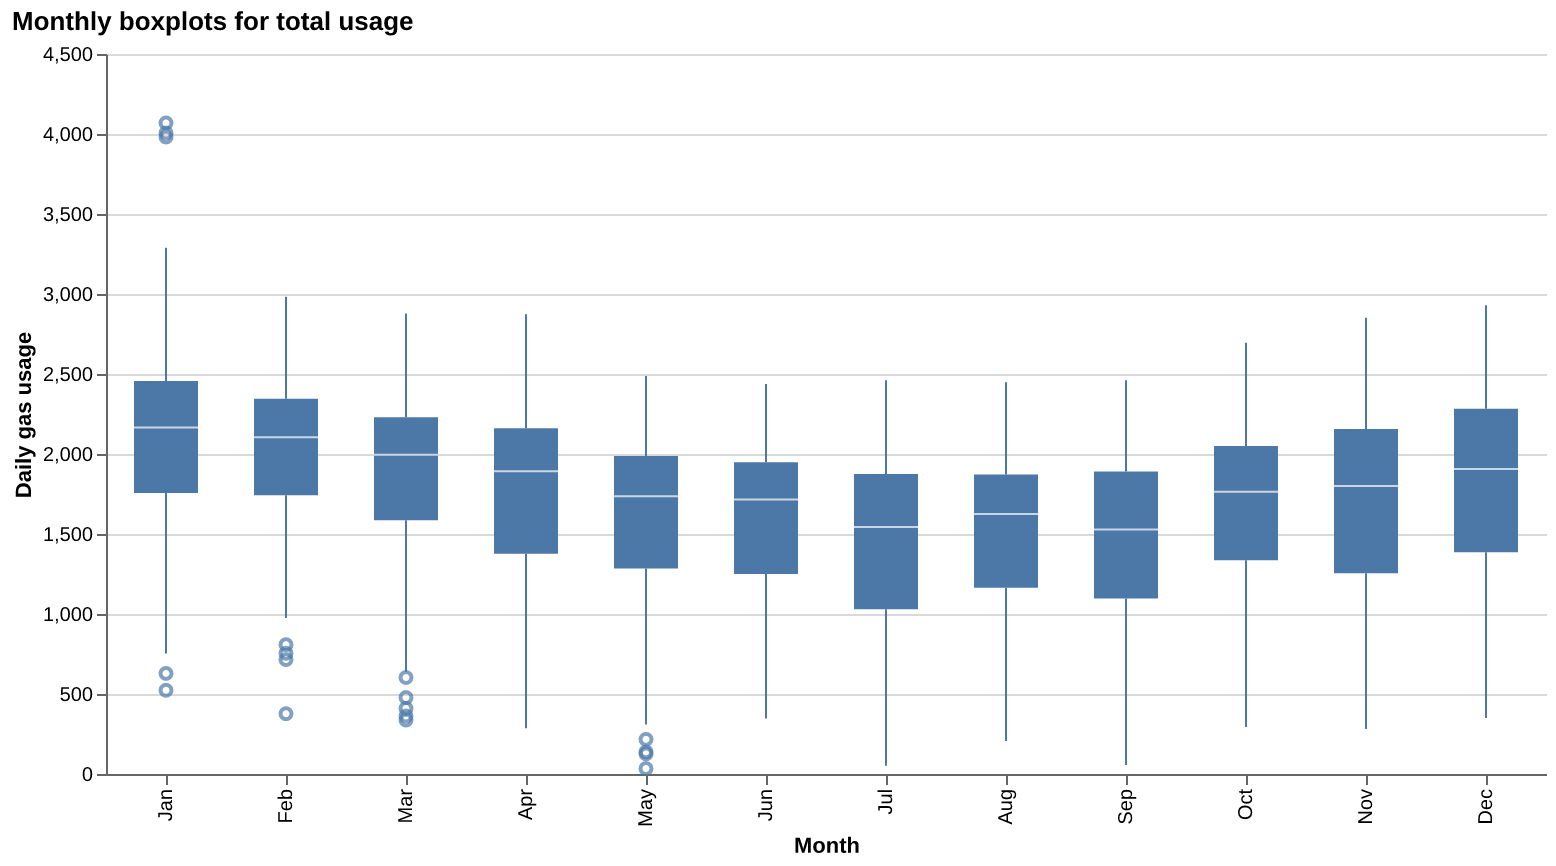
\includegraphics[width=\linewidth]{figures/eda_boxplot_total_usage.png}
    \end{pbox}

  \end{column}

  %% column gap
  \begin{column}{0.019\paperwidth}\end{column}

  %% ==========================================================
  %% COLUMN 2 – Methodology
  %% ==========================================================
  \begin{column}{0.295\paperwidth}

    %% --- Pipeline overview ---
    \begin{pbox}{Pipeline Overview}
      \small
      \begin{center}
        \begin{tikzpicture}[
          node distance=0.55cm,
          box/.style={
            rectangle, rounded corners=5pt,
            draw=navyblue, fill=lightblue, line width=1.2pt,
            text width=6.2cm, align=center,
            minimum height=1.1cm,
            font=\small\bfseries, text=darkgray
          },
          arrow/.style={
            -{Stealth[scale=1.3]}, line width=1.4pt, color=steelblue
          },
          label/.style={font=\footnotesize\itshape, text=midgray}
        ]
          \node[box] (data)  {Raw Gas Meter Data};
          \node[box, below=of data]  (feat)  {EDA \& Feature Engineering};
          \node[box, below=of feat]  (fcast) {Blended Quantile Forecast\\[-1pt]%
                                              \footnotesize P10 / P50 / P95};
          \node[box, below=of fcast] (opt)   {60-Day Rolling LP Optimizer};
          \node[box, below=of opt]   (plan)  {Delivery Nomination Plan};

          \draw[arrow] (data)  -- (feat);
          \draw[arrow] (feat)  -- (fcast);
          \draw[arrow] (fcast) -- (opt);
          \draw[arrow] (opt)   -- (plan);
        \end{tikzpicture}
      \end{center}
    \end{pbox}

    \vspace{0.75cm}

    %% --- Forecasting model ---
    \begin{pbox}{Forecasting Model}
      \small
      \textbf{Architecture:} Blended quantile regression retrained at the
      start of each month. Each quantile (P10/P50/P95) blends a nonlinear
      \emph{GradientBoostingRegressor} (70\%) with a linear
      \emph{QuantileRegressor} solved via HiGHS (30\%).

      \vspace{0.4cm}
      \textbf{Feature groups:}
      \begin{itemize}
        \item Calendar: day-of-week, month, quarter, day-of-year
        \item Business: holiday flags, days-to-end-of-month
        \item Lags: $t{-}1$, $t{-}2$, $t{-}7$, $t{-}30$
        \item Smoothing: rolling mean and std at 7, 14, 30 days
        \item Storage: end-of-month \% history
      \end{itemize}
      \textbf{Production constraint:} only information through day $t{-}2$
      is used to forecast day $t$.

      \vspace{0.5cm}
      \textbf{Benchmark results (Total Usage):}

      \vspace{0.25cm}
      {\footnotesize
      \begin{tabularx}{\linewidth}{@{}Xrrr@{}}
        \toprule
        Model & RMSE & MAE & MAPE \\
        \midrule
        XGBoost                      & 270.5 & 203.8 & 17\% \\
        LightGBM                     & 262.1 & 194.5 & 19\% \\
        CatBoost                     & 258.6 & 191.8 & 20\% \\
        CatBoost + regime + residual & \textbf{258.0} & \textbf{191.8} & 19\% \\
        TimesNet (Usage 1)           & 10.7  & 8.9   &  3\% \\
        PatchTST (Usage 2)           & 255.1 & 184.9 & 20\% \\
        \bottomrule
      \end{tabularx}
      }

      \vspace{0.5cm}
      Lag correlations guided feature selection:

      \vspace{0.2cm}
      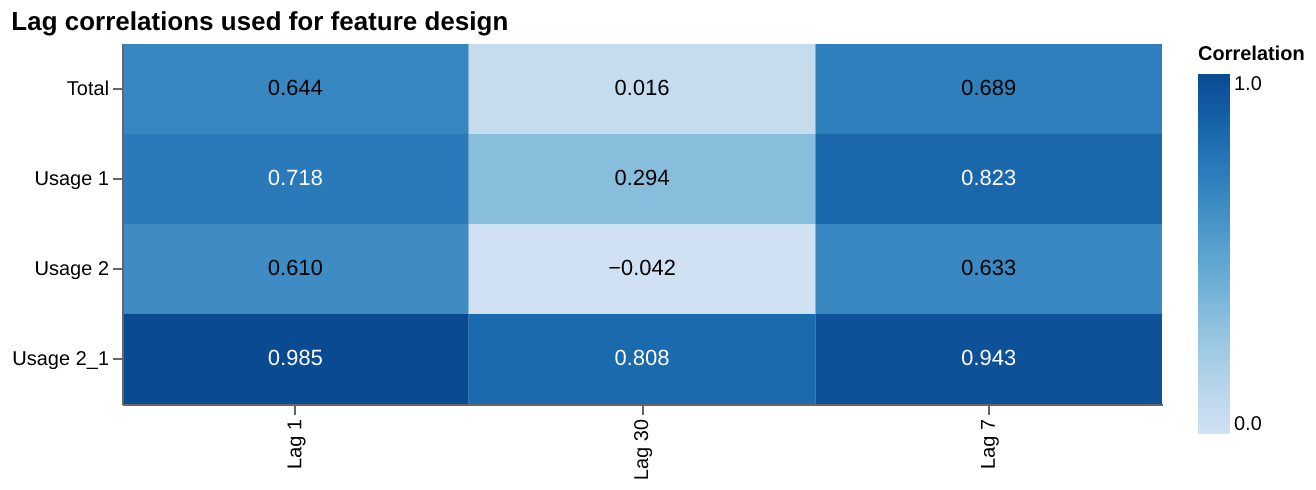
\includegraphics[width=\linewidth]{figures/eda_lag_correlations.png}
    \end{pbox}

    \vspace{0.75cm}

    %% --- Optimization ---
    \begin{pbox}{Optimization Model}
      \small
      \begin{tabularx}{\linewidth}{@{}lX@{}}
        Solver  & \texttt{scipy.optimize.linprog(highs)} \\
        Horizon & Rolling 60-day window \\
        Input   & Conservative P95 usage forecast \\
      \end{tabularx}

      \vspace{0.4cm}
      \textbf{Constraints:}
      \begin{itemize}
        \item Daily injection caps (month-specific \% of 144,841 Dth)
        \item Daily withdrawal caps (month-specific)
        \item Monthly EOM storage bands (0–10\% spring; 85–100\% October)
        \item Mid-month steering target; adaptive seasonal buffers
        \item Feasibility fallback relaxes soft constraints if infeasible
      \end{itemize}
      Using P95 (vs.\ mean) prevents the systematic under-nomination
      that historically caused withdrawal breaches.
    \end{pbox}

  \end{column}

  %% column gap
  \begin{column}{0.019\paperwidth}\end{column}

  %% ==========================================================
  %% COLUMN 3 – Results & Conclusions
  %% ==========================================================
  \begin{column}{0.295\paperwidth}

    %% --- KPI highlight ---
    \begin{pbox}{Key Results — 2022–2024 Backtest}

      \begin{bigkpi}
        \centering
        {\fontsize{74}{78}\selectfont\bfseries\color{resultgreen} 62.9\%}\\[0.2cm]
        {\large\color{white} reduction in daily penalty violations}\\[0.1cm]
        {\normalsize\color{lightblue} 420\ $\rightarrow$\ 156 events}
      \end{bigkpi}

      \vspace{0.6cm}
      {\small
      \begin{tabular}{@{}lrrrr@{}}
        \toprule
        \textbf{KPI} & \textbf{Actual} & \textbf{Opt.}
                     & \boldmath$\Delta$ & \textbf{Reduc.} \\
        \midrule
        Daily violations          & 420 & 156 &
          \textcolor{resultgreen}{$-264$} & \textcolor{resultgreen}{62.9\%} \\
        Monthly EOM violations    & 15  & 15  & $0$    & 0.0\% \\
        Tier 1 cash-out events    & 71  & 22  &
          \textcolor{resultgreen}{$-49$}  & \textcolor{resultgreen}{69.0\%} \\
        Tier 2 cash-out events    & 47  & 25  &
          \textcolor{resultgreen}{$-22$}  & \textcolor{resultgreen}{46.8\%} \\
        Tier 3 cash-out events    & 302 & 109 &
          \textcolor{resultgreen}{$-193$} & \textcolor{resultgreen}{63.9\%} \\
        \bottomrule
      \end{tabular}
      }

      \vspace{0.5cm}
      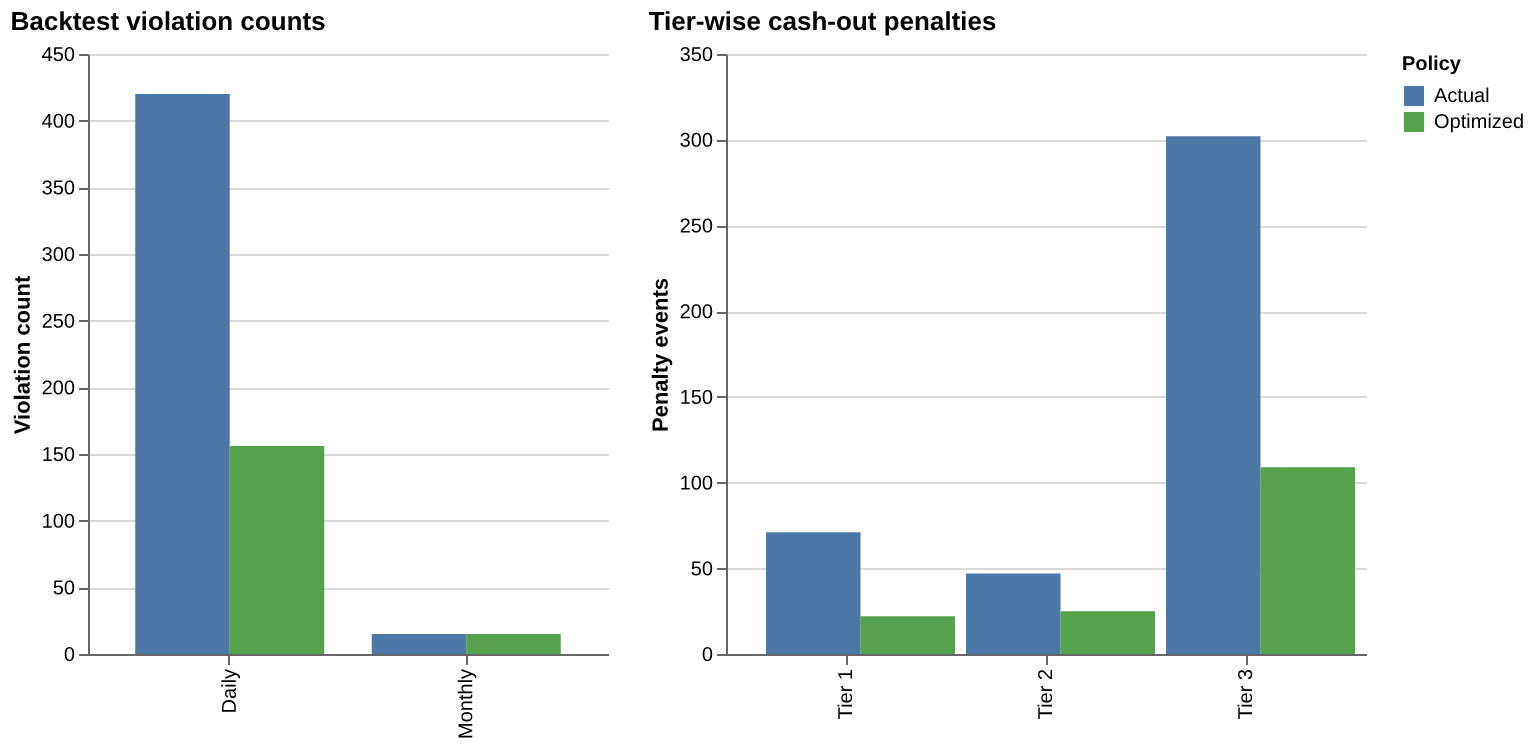
\includegraphics[width=\linewidth]{figures/opt_penalty_summary.png}
    \end{pbox}

    \vspace{0.75cm}

    %% --- Interpretation ---
    \begin{pbox}{Why Optimization Wins}
      \small
      \begin{itemize}
        \item Point-forecast accuracy (RMSE/MAE) was insufficient — tree
              models scored competitively yet still produced daily breaches
        \item \textbf{Quantile forecasts} gave the optimizer a risk-aware
              usage range; P95 avoids the systematic under-nomination that
              triggers withdrawal violations
        \item A \textbf{60-day horizon} lets the LP steer storage toward
              future EOM obligations rather than reacting to each single day
        \item \textbf{Adaptive monthly buffers} addressed asymmetric
              injection/withdrawal risk across seasons
        \item Monthly EOM compliance (15 events) remains unchanged — the
              hardest constraint even after tuning
      \end{itemize}
    \end{pbox}

    \vspace{0.75cm}

    %% --- Conclusions ---
    \begin{pbox}{Conclusions \& Future Work}
      \small
      \textbf{Delivered:} a production-oriented pipeline that handles a
      two-day information lag, converts demand uncertainty into
      P10/P50/P95 scenarios, and chooses penalty-aware delivery nominations
      over a rolling 60-day horizon.

      \vspace{0.45cm}
      \textbf{Core lesson:}
      \begin{callout}
        \small The best model is not the one with the smallest error metric,
        but the one that produces the best \emph{feasible decision} under
        business constraints.
      \end{callout}

      \vspace{0.45cm}
      \textbf{Future directions:}
      \begin{itemize}
        \item Replace violation count objective with dollar-weighted
              penalty cost
        \item Add temperature and weather forecasts as exogenous features
        \item Explore mixed-integer programming for discrete delivery steps
        \item Live deployment with automated monthly retraining and
              live meter feeds
      \end{itemize}
    \end{pbox}

  \end{column}

  %% right margin
  \begin{column}{0.019\paperwidth}\end{column}

\end{columns}

%% ============================================================
%% FOOTER
%% ============================================================
\vspace{0.8cm}
\begin{beamercolorbox}[wd=\paperwidth, ht=2.6cm, sep=0.55cm]{posterfooter}
  \centering\small
  \textbf{Tools:} Python \textbullet{} Polars \textbullet{} Altair
  \textbullet{} scikit-learn \textbullet{} SciPy HiGHS \textbullet{} Marimo
  \quad$|$\quad
  \textbf{Data:} 3,410 daily gas meter records, Aug 2015 – Nov 2024
  \quad$|$\quad
  \textbf{Backtest:} Jan 2022 – Sep 2024
\end{beamercolorbox}

\end{frame}
\end{document}
